%!Tex root = Report.tex
\Section{Results}
\SubSection{Performance}
This section presents results of performance comparison between Neo4j and GraphLab. 
\begin{itemize}
\item Figure \ref{fig:dense-edges} and \ref{fig:sparse-edges} show the comparison between Neo4j and GraphLab with varying number of edges in the dataset. GraphLab performs better than Neo4j over the entire range of dataset generated.
\item Similar comparison with the number of nodes per dataset is shown in plots \ref{fig:dense-nodes} and \ref{fig:sparse-nodes}. Over the small dataset, the relative difference between GraphLab and Neo4j is high, however it reduces as the data scales up.
\item Figure \ref{fig:neo4j-sparse-dense} and \ref{fig:graphlab-sparse-dense} show that the execution time for a sparse dataset is always smaller than dense datasets. This is expected because dense graphs have high number of neighbors which lead to higher query processing time.
\end{itemize}
\SubSection{Cluster Purity}
This section introduces one of the external criteria of clustering quality. Purity is a simple and transparent evaluation measure. To compute purity, each cluster is assigned to the class which is most frequent in the cluster, and then the accuracy of this assignment is measured by counting the number of correctly assigned documents and dividing by N. Here, class is the set of clusters we already know in the synthetic input data for clustering and N is the total number of nodes in the graph. Formally
\begin{equation}
purity(\Omega, C ) = \frac{1}{N}\sum_{k} max_{j}|w_{k} \bigcap c_{j}|
\end{equation}
where $\Omega = \{w_{1}, w_{2},....,w_{k}\}$ is the set of clusters and $C=\{c_{1},c_{2},...,c{j}\}$ is the set of classes.
High purity is easy to achieve when the number of clusters is large - in particular, purity is 1 if each document gets its own cluster. However, we are getting number of resulting clusters almost equal to the number of gold standard clusters. Hence this measure is reasonable here to judge performance of our clustering algorithm.\\
\textbf{NOTE:} We know the number of actual clusters in the synthetic data generated from networkx. Therefore we will call it as gold standard data.

\begin{itemize}
\item Performance of our implementation is better on dense graph as compared to sparse graph, which is expected considering nodes are scattered in sparse graph.
\item Average clustering purity for dense graph having number of edges $> 200,000$ is $0.92$.
\item Average clustering purity for sparse graph having number of edges $> 200,000$ is $0.84$.
\item For smaller datasets having edge counts between $20,000$ to $100,000$, we are achieving nearly perfect clustering. Clustering coefficient for them is $>0.98$ with same number of clusters/ classes in output as in the gold data.
\end{itemize}

	\begin{figure}
		\begin{minipage}{.5\textwidth}
			\centering
			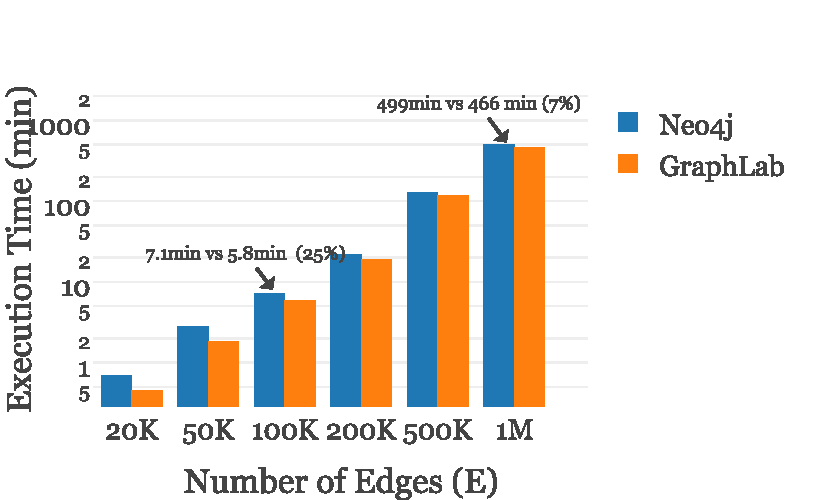
\includegraphics[scale=0.5]{Graphs/dense-edges.pdf}
			\caption{Dense datasets - Neo4j vs GraphLab\label{fig:dense-edges}}
		\end{minipage}
		\begin{minipage}{.5\textwidth}
			\centering
			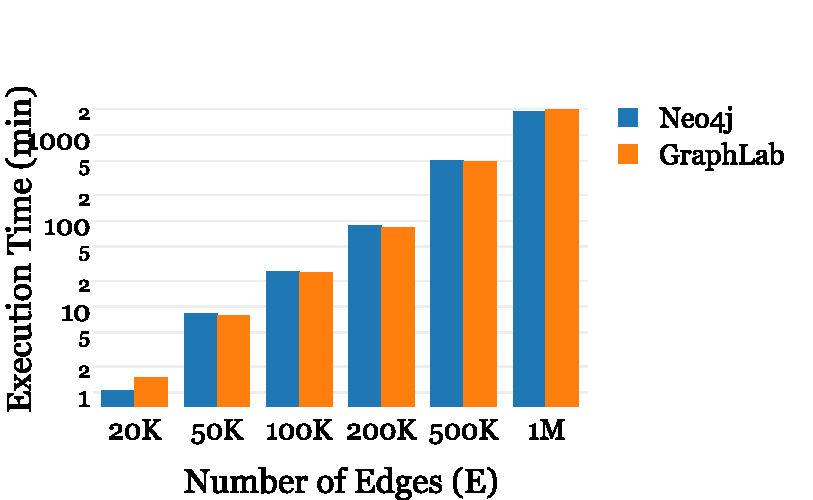
\includegraphics[scale=0.5]{Graphs/sparse-edges.pdf}
			\caption{Sparse datasets - Neo4j vs GraphLab\label{fig:sparse-edges}}
		\end{minipage}
	\end{figure}
	
	
	\begin{figure}
		\begin{minipage}{.5\textwidth}
			\centering
			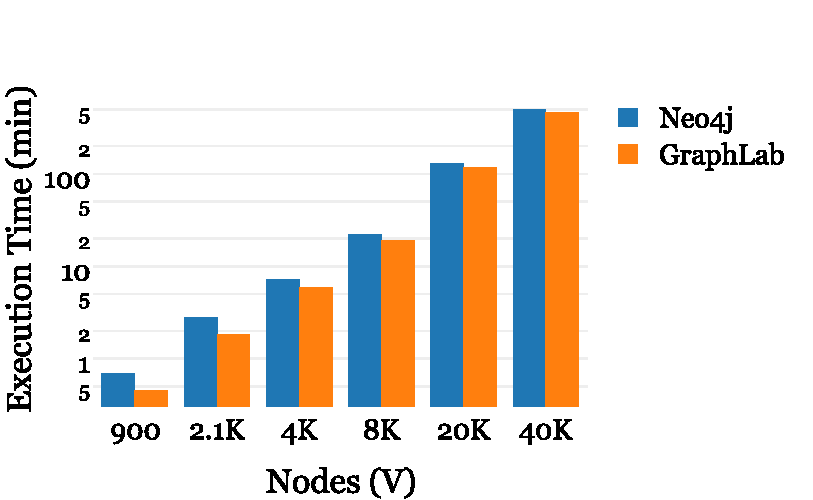
\includegraphics[scale=0.5]{Graphs/dense-nodes.pdf}
			\caption{Dense datasets - Neo4j vs GraphLab\label{fig:dense-nodes}}
		\end{minipage}
		\begin{minipage}{.5\textwidth}
			\centering
			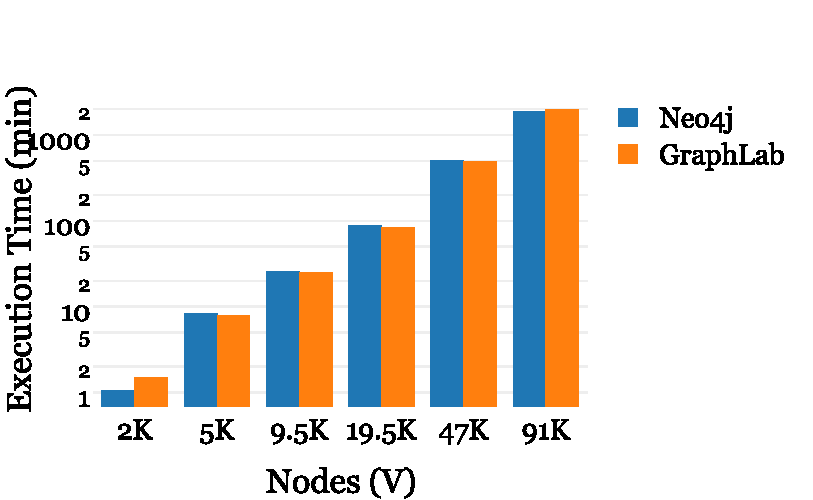
\includegraphics[scale=0.5]{Graphs/sparse-nodes.pdf}
			\caption{Sparse datasets - Neo4j vs GraphLab\label{fig:sparse-nodes}}
		\end{minipage}
	\end{figure}
	
	\begin{figure}
		\begin{minipage}{.5\textwidth}
			\centering
			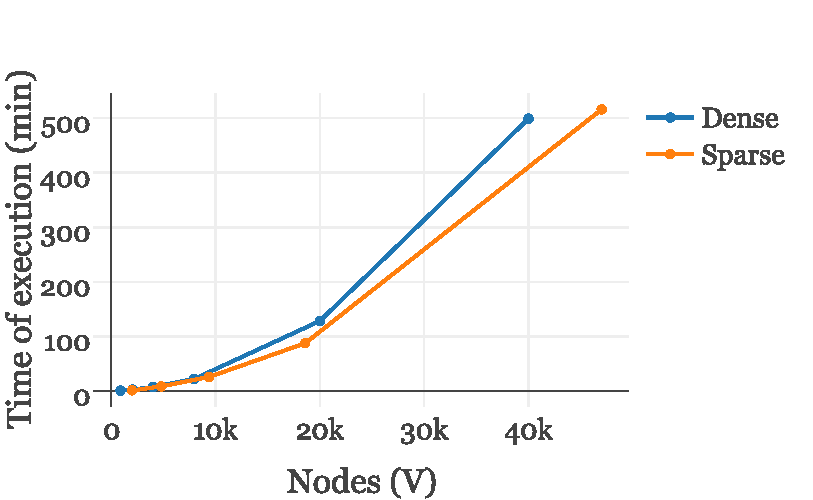
\includegraphics[scale=0.5]{Graphs/neo4j-sparse-dense.pdf}
			\caption{Neo4j - Dense vs Sparse datasets\label{fig:neo4j-sparse-dense}}
		\end{minipage}
		\begin{minipage}{.5\textwidth}
			\centering
			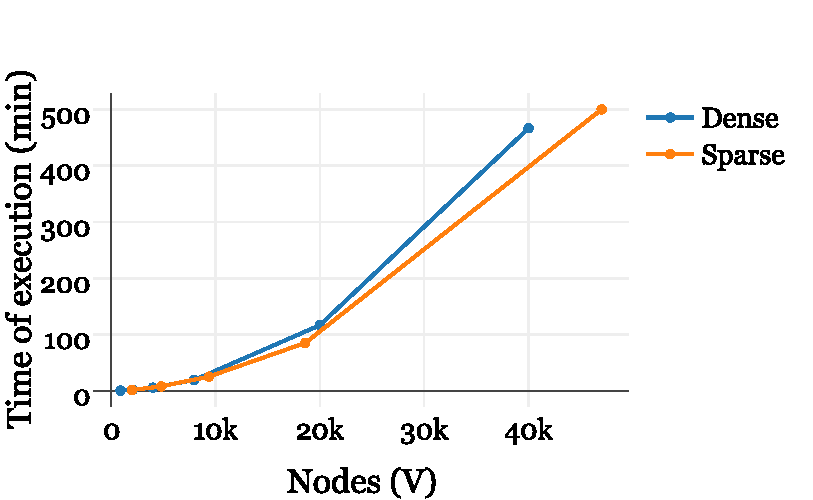
\includegraphics[scale=0.5]{Graphs/graphlab-sparse-dense.pdf}
			\caption{GraphLab - Dense vs Sparse datasets\label{fig:graphlab-sparse-dense}}
		\end{minipage}
	\end{figure}
	

\SubSection{Clustering on real world dataset: Facebook}
This section presents clustering performance of real world social network Facebook \cite{facebookdata} from Stanford Large Network Dataset Collection \cite{snap}.\\
\\
\textbf{Facebook Dataset Details:}
\begin{itemize}
	\item
	Nodes: 4039
	\item
	Edges: 88234
	\item
	Average clustering coefficient:	0.6055
	\item
	Number of triangles:	1612010
\end{itemize}
\noindent
\textbf{Facebook Dataset Results:}
\begin{itemize}
	\item
	Total number of clusters detected: 8
	\item
	Total Execution Time (Neo4j): 11.3 minutes
	\item
	Total Execution Time (GraphLab): 9.5 minutes
	\item
	List of clusters with number of nodes in them:\\
	Cluster-1 Nodes:1368\\
	Cluster-2 Nodes:770\\
	Cluster-3 Nodes:753\\
	Cluster-4 Nodes:590\\
	Cluster-5 Nodes:316\\
	Cluster-6 Nodes:211\\
	Cluster-7 Nodes:21\\
	Cluster-8 Nodes:10	
\end{itemize}
\begin{figure}
	\centering
	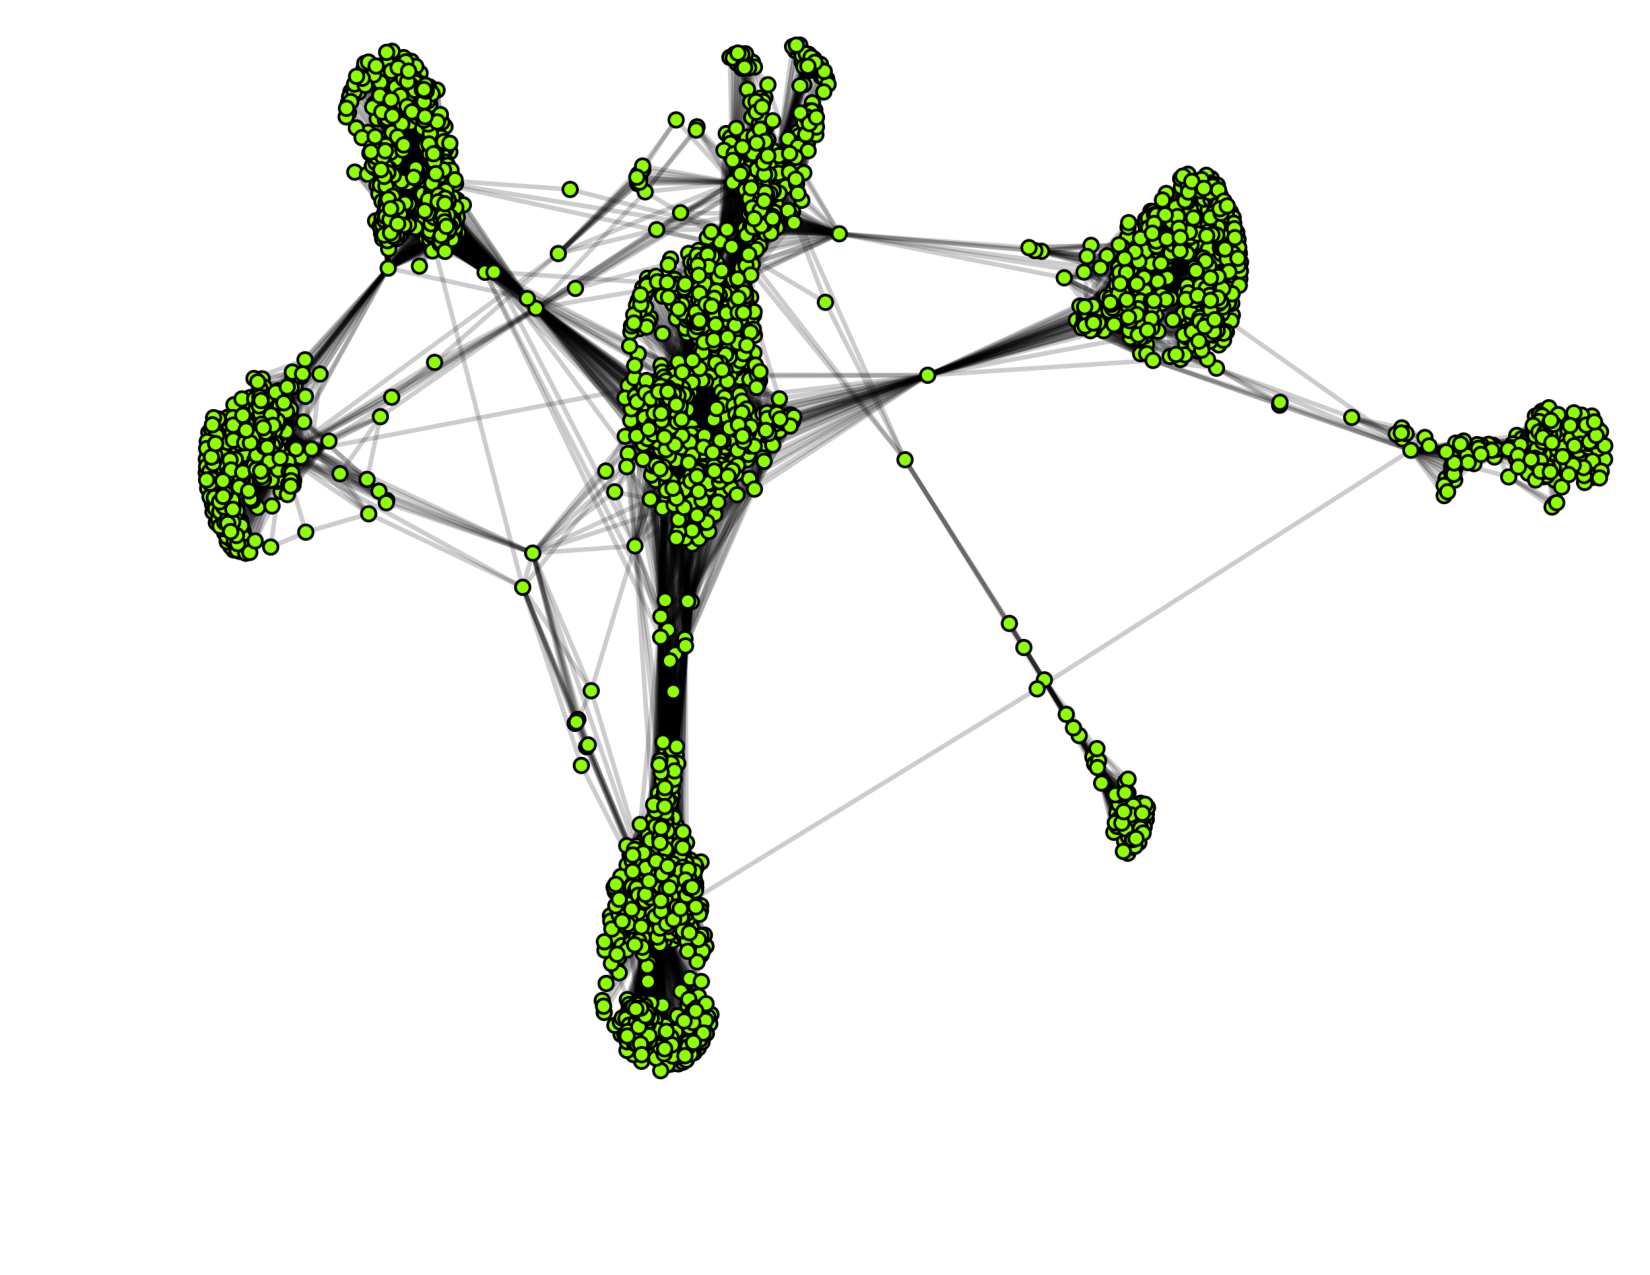
\includegraphics[scale=0.4, trim=0 0 20 0]{Images/before_facebook.pdf}
	\caption{Facebook Dataset - Before Clustering\label{fig:fb-before}}
\end{figure}
\begin{figure}
	\centering
	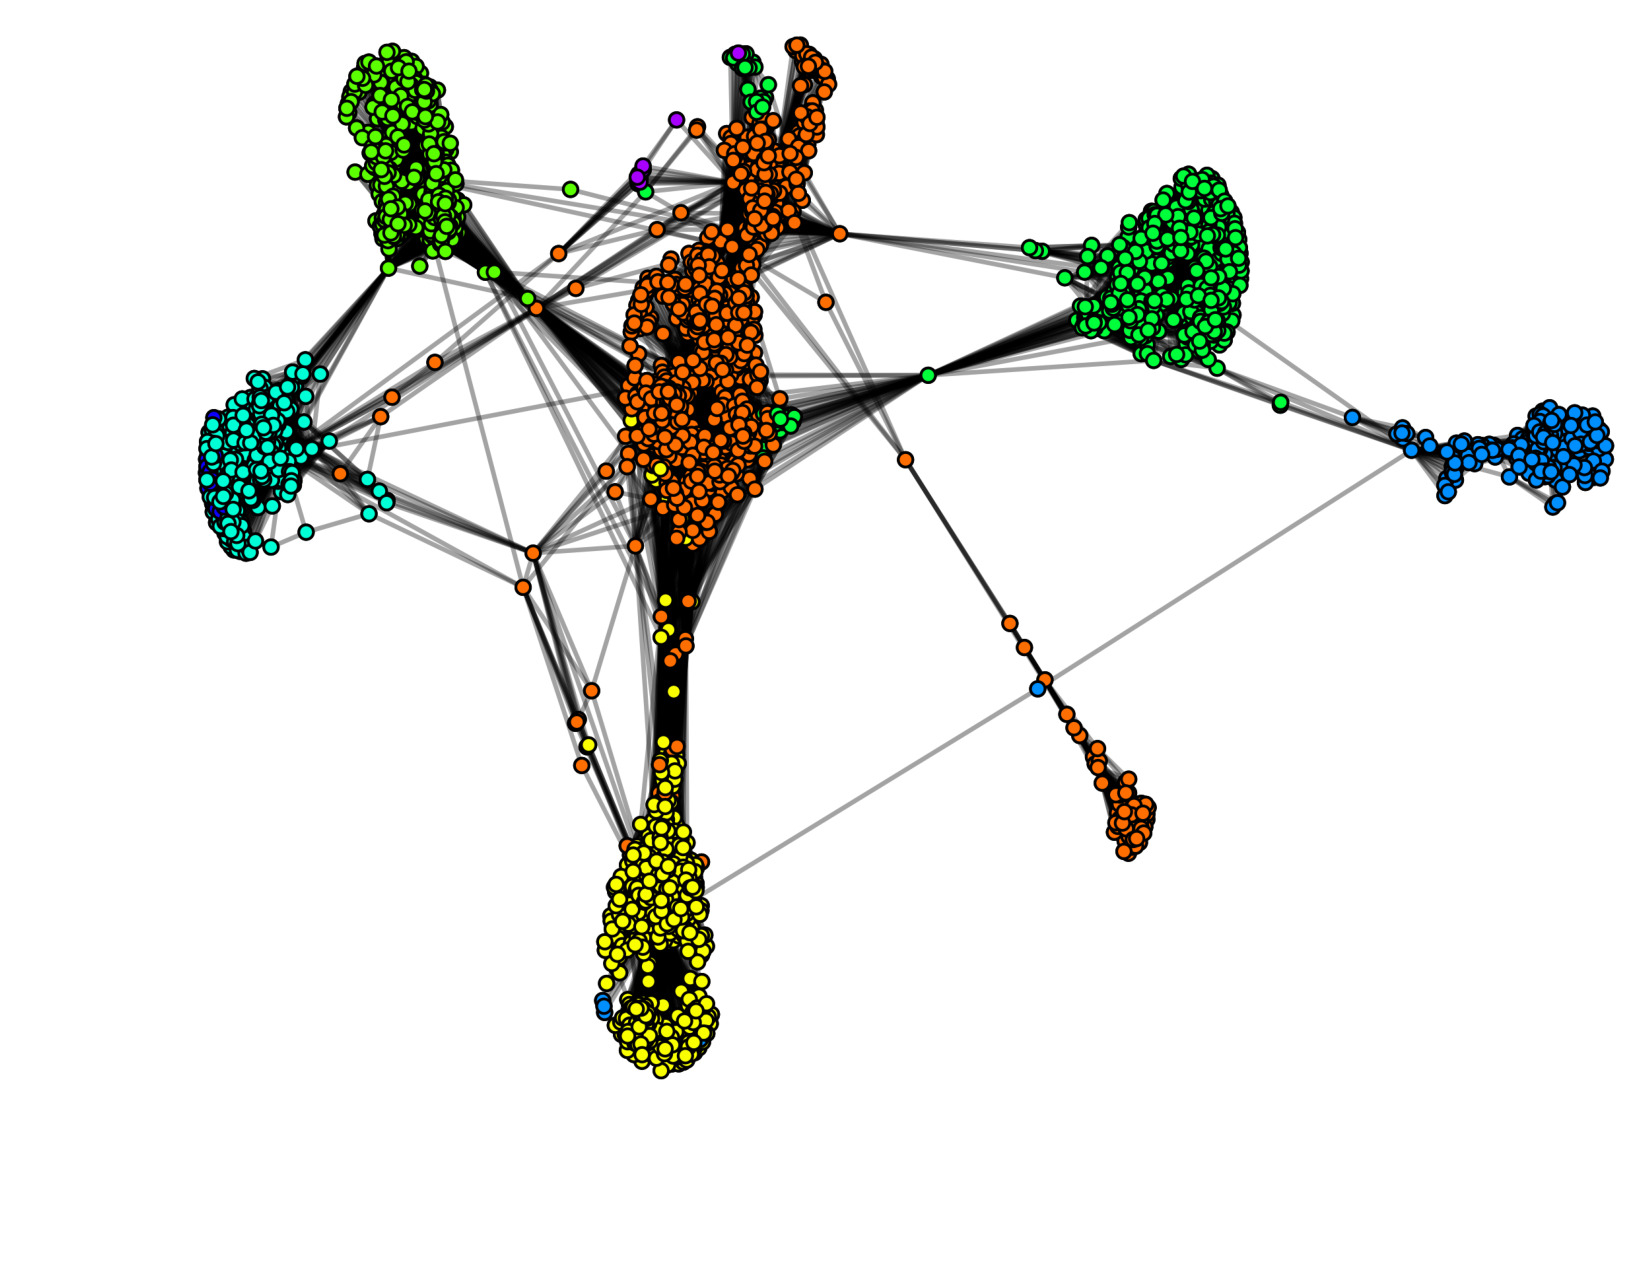
\includegraphics[scale=0.4, trim=0 0 20 0]{Images/after_facebook.pdf}
	\caption{Facebook Dataset - After Clustering (Neo4j/GraphLab)\label{fig:fb-after}}
\end{figure}